\chapter{Desarrollo. Entregas e iteraciones}
\label{ch:desarrollo}
Este capítulo recoge el proceso de desarrollo del juego, en el que se detallan las diferentes entregas e iteraciones, así como los resultados de estas.

\section{Entrega 0}
En esta entrega se ha llevado a cabo una prueba de viabilidad del proyecto, en la que se ha comprobado como funciona el SDK ARCore, y que posibilidades ofrece. La prueba que se llevó a cabo consistía en asociar diferentes elementos 3D a diferentes imágenes.\\

En la Figura \ref{figura-demo-tablero} se puede observar la demo en funcionamiento, en ella la aplicación reconoce la imagen del tablero de juego y le asocia un cubo 3D que se muestra en el centro del tablero.

\begin{figure}[h]
  \centering
  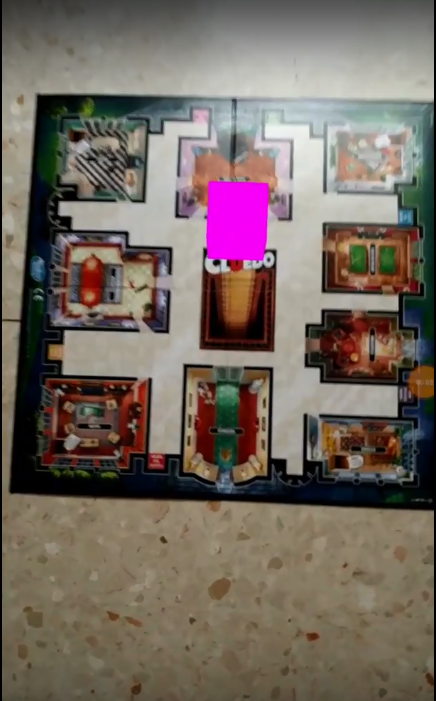
\includegraphics[scale=0.4]{demo-tablero}
  \caption{Imagen que muestra la demo en la que hay un objeto 3D asociado al tablero de juego.}
  \label{figura-demo-tablero}
\end{figure}

En la Figura \ref{figura-demo-imagenes} se puede observar la demo en funcionamiento, en ella la aplicación reconoce la imagen del tablero y las de diferentes habitaciones y asocia diferentes elementos 2D a cada una de las imágenes.

\begin{figure}[h]
  \centering
  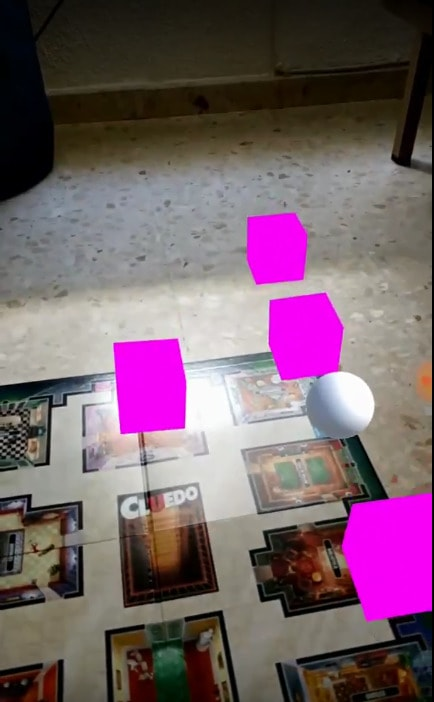
\includegraphics[scale=0.4]{demo-imagenes}
  \caption{Imagen que muestra la demo en la que hay objetos 3D asociados al tablero y diferentes habitaciones.}
  \label{figura-demo-imagenes}
\end{figure}

\FloatBarrier

\subsection{Primera iteración}
En esta iteración se ha realizado la demo que se ha mostrado en la \textbf{Entrega 0}.\\

Por otro lado, se ha llevado a cabo una versión inicial del documento de diseño de videojuegos (GDD), que se encuentra en el Apéndice \ref{documento-diseño-videojuegos}, dejando definidos los conceptos iniciales.\\

También se han llevado a cabo las historias de usuario que definen las situaciones en las que un usuario se encontrará cuando quiera llevar a cabo una acción en el juego, estas historias se pueden encontrar en el Apéndice \ref{historias-usuario}, y la lista con las historias de usuario se puede encontrar en el Capítulo \ref{ch:plan}, en la sección "Historias de usuario".\\

Por último en esta iteración se llevó la recopilación de elementos 3D que se utilizarían en el juego.

\subsection{Conclusiones}
Al realizarse la prueba de viabilidad asociando figuras 3D con realidad aumentada a imagenes escaneadas, se pudo comprobar que la realidad aumentada es muy interesante para aplicar en juegos de mesa por las posibilidades que ofrece, permitiendo un realismo que solo un juego de mesa real físico puede alcanzar. Por otro lado se vio que era posible utilizar ARCore para desarrollar un juego junto con el motor Unity, y obtener un resultado satisfactorio.\\

Por otro lado se comprobó que ARCore aun no permite el seguimiento de imagenes en movimiento, por lo que si se mueve el tablero hasta que no lo vuelva a detectar parado no cambia los modelos 3D a esa nueva posición, pero esta característica no era necesaria para nuestro proyecto, ya que al ser un juego de mesa no habrá mucho movimiento.

\section{Entrega 1}
En esta entrega se han llevado a cabo bocetos del juego, y pruebas heurísticas y de usuario sobre estos.

%%%%%%%%%%%%%%%%%%%%%%%%%%%%%%%%%%%%%%%%%%%%%%%%%% BOCETOS %%%%%%%%%%%%%%%%%%%%%%%%%%%%%%%%%%%%%%%%%%%%%%%%%%%%%%
\subsection{Bocetos}
Se han creado bocetos que representan la idea inicial del juego y cómo serán sus diferentes pantallas e interfaces, de forma que se puedan utilizar para llevar a cabo pruebas sobre ellos, dichas pruebas incluyen pruebas heurísticas realizadas por el desarrollador y pruebas se usabilidad con usuarios reales, para así saber que esta bien y que no en los bocetos y mejorar el diseño del juego.\\

En la Figura \ref{figura-b1} se puede ver el boceto creado para la pantalla inicial en la que se seleccionará los personajes con los que se quiere jugar:

\begin{figure}[h]
  \centering
  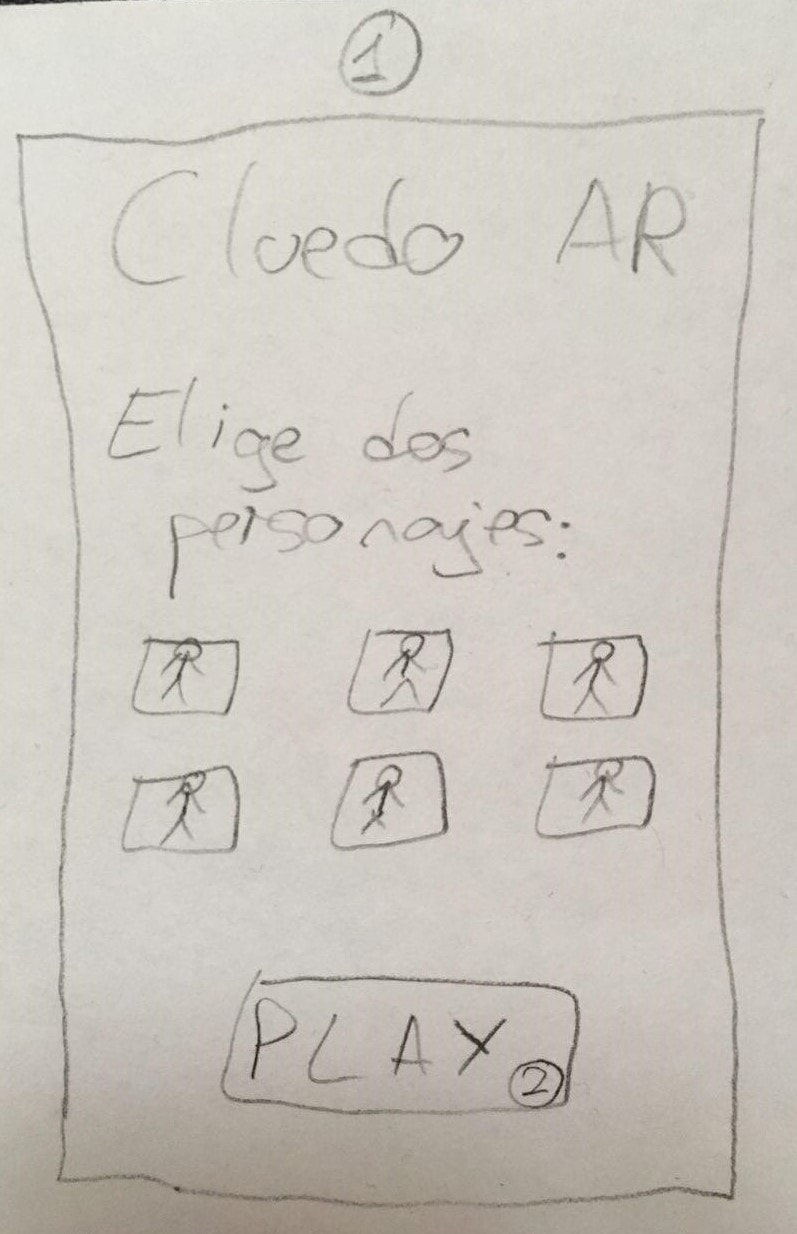
\includegraphics[scale=0.2]{b1}
  \caption{Imagen que muestra la interfaz de la pantalla inicial del juego.\protect\footnotemark}
  \label{figura-b1}
\end{figure}

\newpage

En la Figura \ref{figura-b2} se puede ver el boceto creado para la pantalla de instrucciones:

\begin{figure}[h]
  \centering
  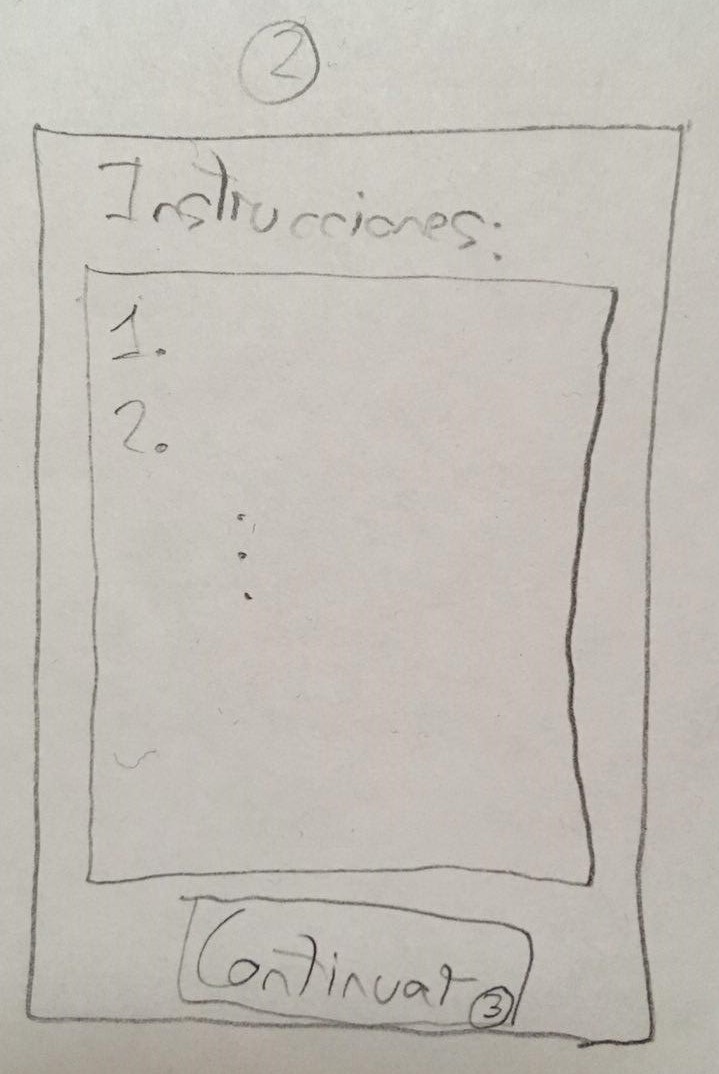
\includegraphics[scale=0.2]{b2}
  \caption{Imagen que muestra la interfaz de la pantalla de instrucciones del juego.\protect\footnotemark}
  \label{figura-b2}
\end{figure}

El resto de los bocetos se pueden encontrar en la sección \ref{bocetos} del Anexo.

\subsection{Pruebas heurísticas}
\begin{itemize}

  \item \textbf{Principio 1: Visibilidad del estado del sistema.}\\
  La puntuación es de 7, el usuario está bien informado de lo que ocurre actualmente en el sistema, se muestra siempre que es necesario el botón “home” o el botón “atrás”, pero se puede mejorar, por ejemplo, indicando que se están escaneando imágenes mientras mueves el dispositivo sobre el tablero.

  \item \textbf{Principio 2: Correspondencia entre el sistema y el mundo real.}\\
  La puntuación es de 10, las opciones en los menús están ordenadas de forma lógica y el lenguaje que el juego utiliza es un lenguaje común al usuario del juego.

  \item \textbf{Principio 3: Control y libertad del usuario.}\\
  La puntuación es de 7, ya que en la mayoría de pantallas el usuario es libre de ir hacia adelante o hacia atrás, pero en instrucciones el usuario puede avanzar al juego pero no volver a la pantalla de inicio. Además, como se puede ver en la pantalla 6, para hacer apuntes, el botón de retroceso está en la zona derecha de la pantalla, pudiendo confundir esto al usuario, ya que es una función de retroceso no de avance.

  \item \textbf{Principio 4: Consistencia y estándares.}\\
  La puntuación es de 7, ya que es bastante consistente, pero en la pantalla que indica el ganador aparece el botón “home” como en otras pantallas, pero se muestra en una posición distinta, lo que resulta confuso al usuario habría que moverlo a la posición que ocupa siempre o utilizar otro botón.

  \item \textbf{Principio 5: Prevención de errores.}\\
  La puntuación es de 10, el diseño es bastante cuidadoso para la prevención de errores y el correcto tratamiento de estos.

  \item \textbf{Principio 6: Minimizar la carga de memoria del usuario.}\\
  La puntuación es de 10, el usuario no necesita recordar nada en ningún momento, todo se muestra de forma apropiada para que no suponga ninguna memorización al usuario.

  \item \textbf{Principio 7: Personalización y atajos.}
  La puntuación es de 10, la aplicación no dispone de personalización o atajos, pero no son necesarios en esta, por lo que no afecta a la experiencia de usuario.

  \item \textbf{Principio 8: Eficiencia de uso y rendimiento.}
  La puntuación es de 8, la aplicación está bien optimizada para que al usuario le resulte sencillo y rápido llevar a cabo cualquier tarea, pero si es cierto que algunos botones que se utilizan con mucha frecuencia no están en las posiciones óptimas.

  \item \textbf{Principio 9: Estética y diseño minimalista.}
  La puntuación es de 10, la información que se muestra en la aplicación es la necesaria para que el usuario pueda jugar con la mejor experiencia de usuario posible, no hay exceso o falta de información.

  \item \textbf{Principio 10: Ayuda al usuario a reconocer, diagnosticar y recuperarse de errores.}
  La puntuación es de 10, ya que no hay posibilidad de que ocurran errores en el juego.

  \item \textbf{Principio 11: Ayuda y documentación.}
  La puntuación es de 10, ya que antes de comenzar cada partida se muestra al usuario unas instrucciones de cómo funciona el juego.

  \item \textbf{Principio 12: Interacción física y ergonomía.}
  La puntuación es de 10, ya que los botones son fácilmente diferenciables y están en una posición cómoda para el usuario, teniendo en cuenta que al ser un juego utilizará las dos manos para usar el dispositivo móvil.

\end{itemize}

\subsection{Pruebas de usabilidad}
Las tablas que contienen la información obtenida en estas pruebas de usabilidad se encuentran en la sección \ref{tablas-usabilidad-bocetos} del Anexo.

\begin{itemize}
  \item \textbf{Usuario 1}

  \textbf{Pre Test}

  \begin{enumerate}
    \item Edad: 18
    \item Dispone de un dispositivo móvil: Sí
    \item Con qué frecuencia utiliza su dispositivo móvil: Varias veces al dia
    \item Con qué frecuencia juega a juegos de mesa: Varias veces al año
    \item Con qué frecuencia juega a juegos en su móvil: Varias veces a la semana
  \end{enumerate}

  \textbf{Test}: Los resultados del test de usabilidad sobre el Usuario 1 se encuentran en la Tabla \ref{tabla-bocetos-usuario1}


  \item \textbf{Usuario 2}

  \textbf{Pre Test}

  \begin{enumerate}
    \item Edad: 57
    \item Dispone de un dispositivo móvil: Sí
    \item Con qué frecuencia utiliza su dispositivo móvil: Varias veces al día
    \item Con qué frecuencia juega a juegos de mesa: Varias veces al año
    \item Con qué frecuencia juega a juegos en su móvil: Varias veces al día
  \end{enumerate}

  \textbf{Test}: Los resultados del test de usabilidad sobre el Usuario 2 se encuentran en la Tabla \ref{tabla-bocetos-usuario2}


  \item \textbf{Usuario 3}

  \textbf{Pre Test}

  \begin{enumerate}
    \item Edad: 26
    \item Dispone de un dispositivo móvil: Sí
    \item Con qué frecuencia utiliza su dispositivo móvil: Varias veces al dia
    \item Con qué frecuencia juega a juegos de mesa: Una vez al mes como máximo
    \item Con qué frecuencia juega a juegos en su móvil: Casi nunca
  \end{enumerate}

  \textbf{Test}: Los resultados del test de usabilidad sobre el Usuario 3 se encuentran en la Tabla \ref{tabla-bocetos-usuario3}

\subsection{Segunda iteración}
En esta iteración se ha llevado a cabo los bocetos, que se pueden encontrar en el Apéndice \ref{bocetos}, esos nos servirán para crear un primer concepto de como serán las interfaces de las diferentes pantallas del juego.\\

También se llevaron a cabo pruebas heuristicas con el desarrollador, para comprobar los posibles errores y mejoras de los bocetos. Los resultados de estas pruebas se pueden encontrar en la \textbf{Entrega 1}.\\

Por último, se realizaron pruebas con usuarios, poniendoles en situación se les indicaba la tarea que tenian que hacer, y se fueron apuntando los problemas que estos tenian, detectando así elementos que mejorar en los bocetos. Los resultados de estas pruebas de usabilidad se encuentran en las Tablas \ref{tabla-bocetos-usuario1}, \ref{tabla-bocetos-usuario2} y \ref{tabla-bocetos-usuario3}.\\

Con toda la información obtenida de la realización de los bocetos y pruebas de usuario se han modificado aspectos del GDD, adaptando el funcionamiento del juego a las necesidades de los jugadores, y ajustando los perfiles de forma más realista al de los posibles futuros jugadores del juego. El documento de diseño del videojuego se puede encontrar en el Apéndice \ref{documento-diseño-videojuegos}.

\subsection{Conclusiones}
Durante las pruebas de usabilidad pruebas hemos podido comprobar que la interfaz de la aplicación es amigable para los usuarios, que si bien han detectado algunos fallos, que serán solventados en el desarrollo del juego, por lo general han sabido realizar todas las tareas sin dificultad, desenvolviéndose con rapidez.\\

También se ha podido comprobar el interés de los usuarios por el funcionamiento de la realidad aumentada, resultándoles algo sorprendente y que sin duda tenían ganas de probar en las siguientes pruebas de usabilidad, lo que denota la esperada expectación de los usuarios de juegos y en general de dispositivos móviles sobre la realidad aumentada y las novedosas experiencias que esta aportará al ámbito de los dispositivos móviles.

\section{Entrega 2}
En esta entrega se ha completado la pantalla inicial que permite seleccionar los personajes de los jugadores, la pantalla de instrucciones que explica el funcionamiento del juego y la pantalla de juego en la que se podrá escanear el tablero y se mostrarán los modelos 3D que se utilizarán en el juego sobre dicho tablero.\\

En la Figura \ref{figura-inicial-1} se puede observar la pantalla de inicio sin personajes seleccionados.

\begin{figure}[h]
  \centering
  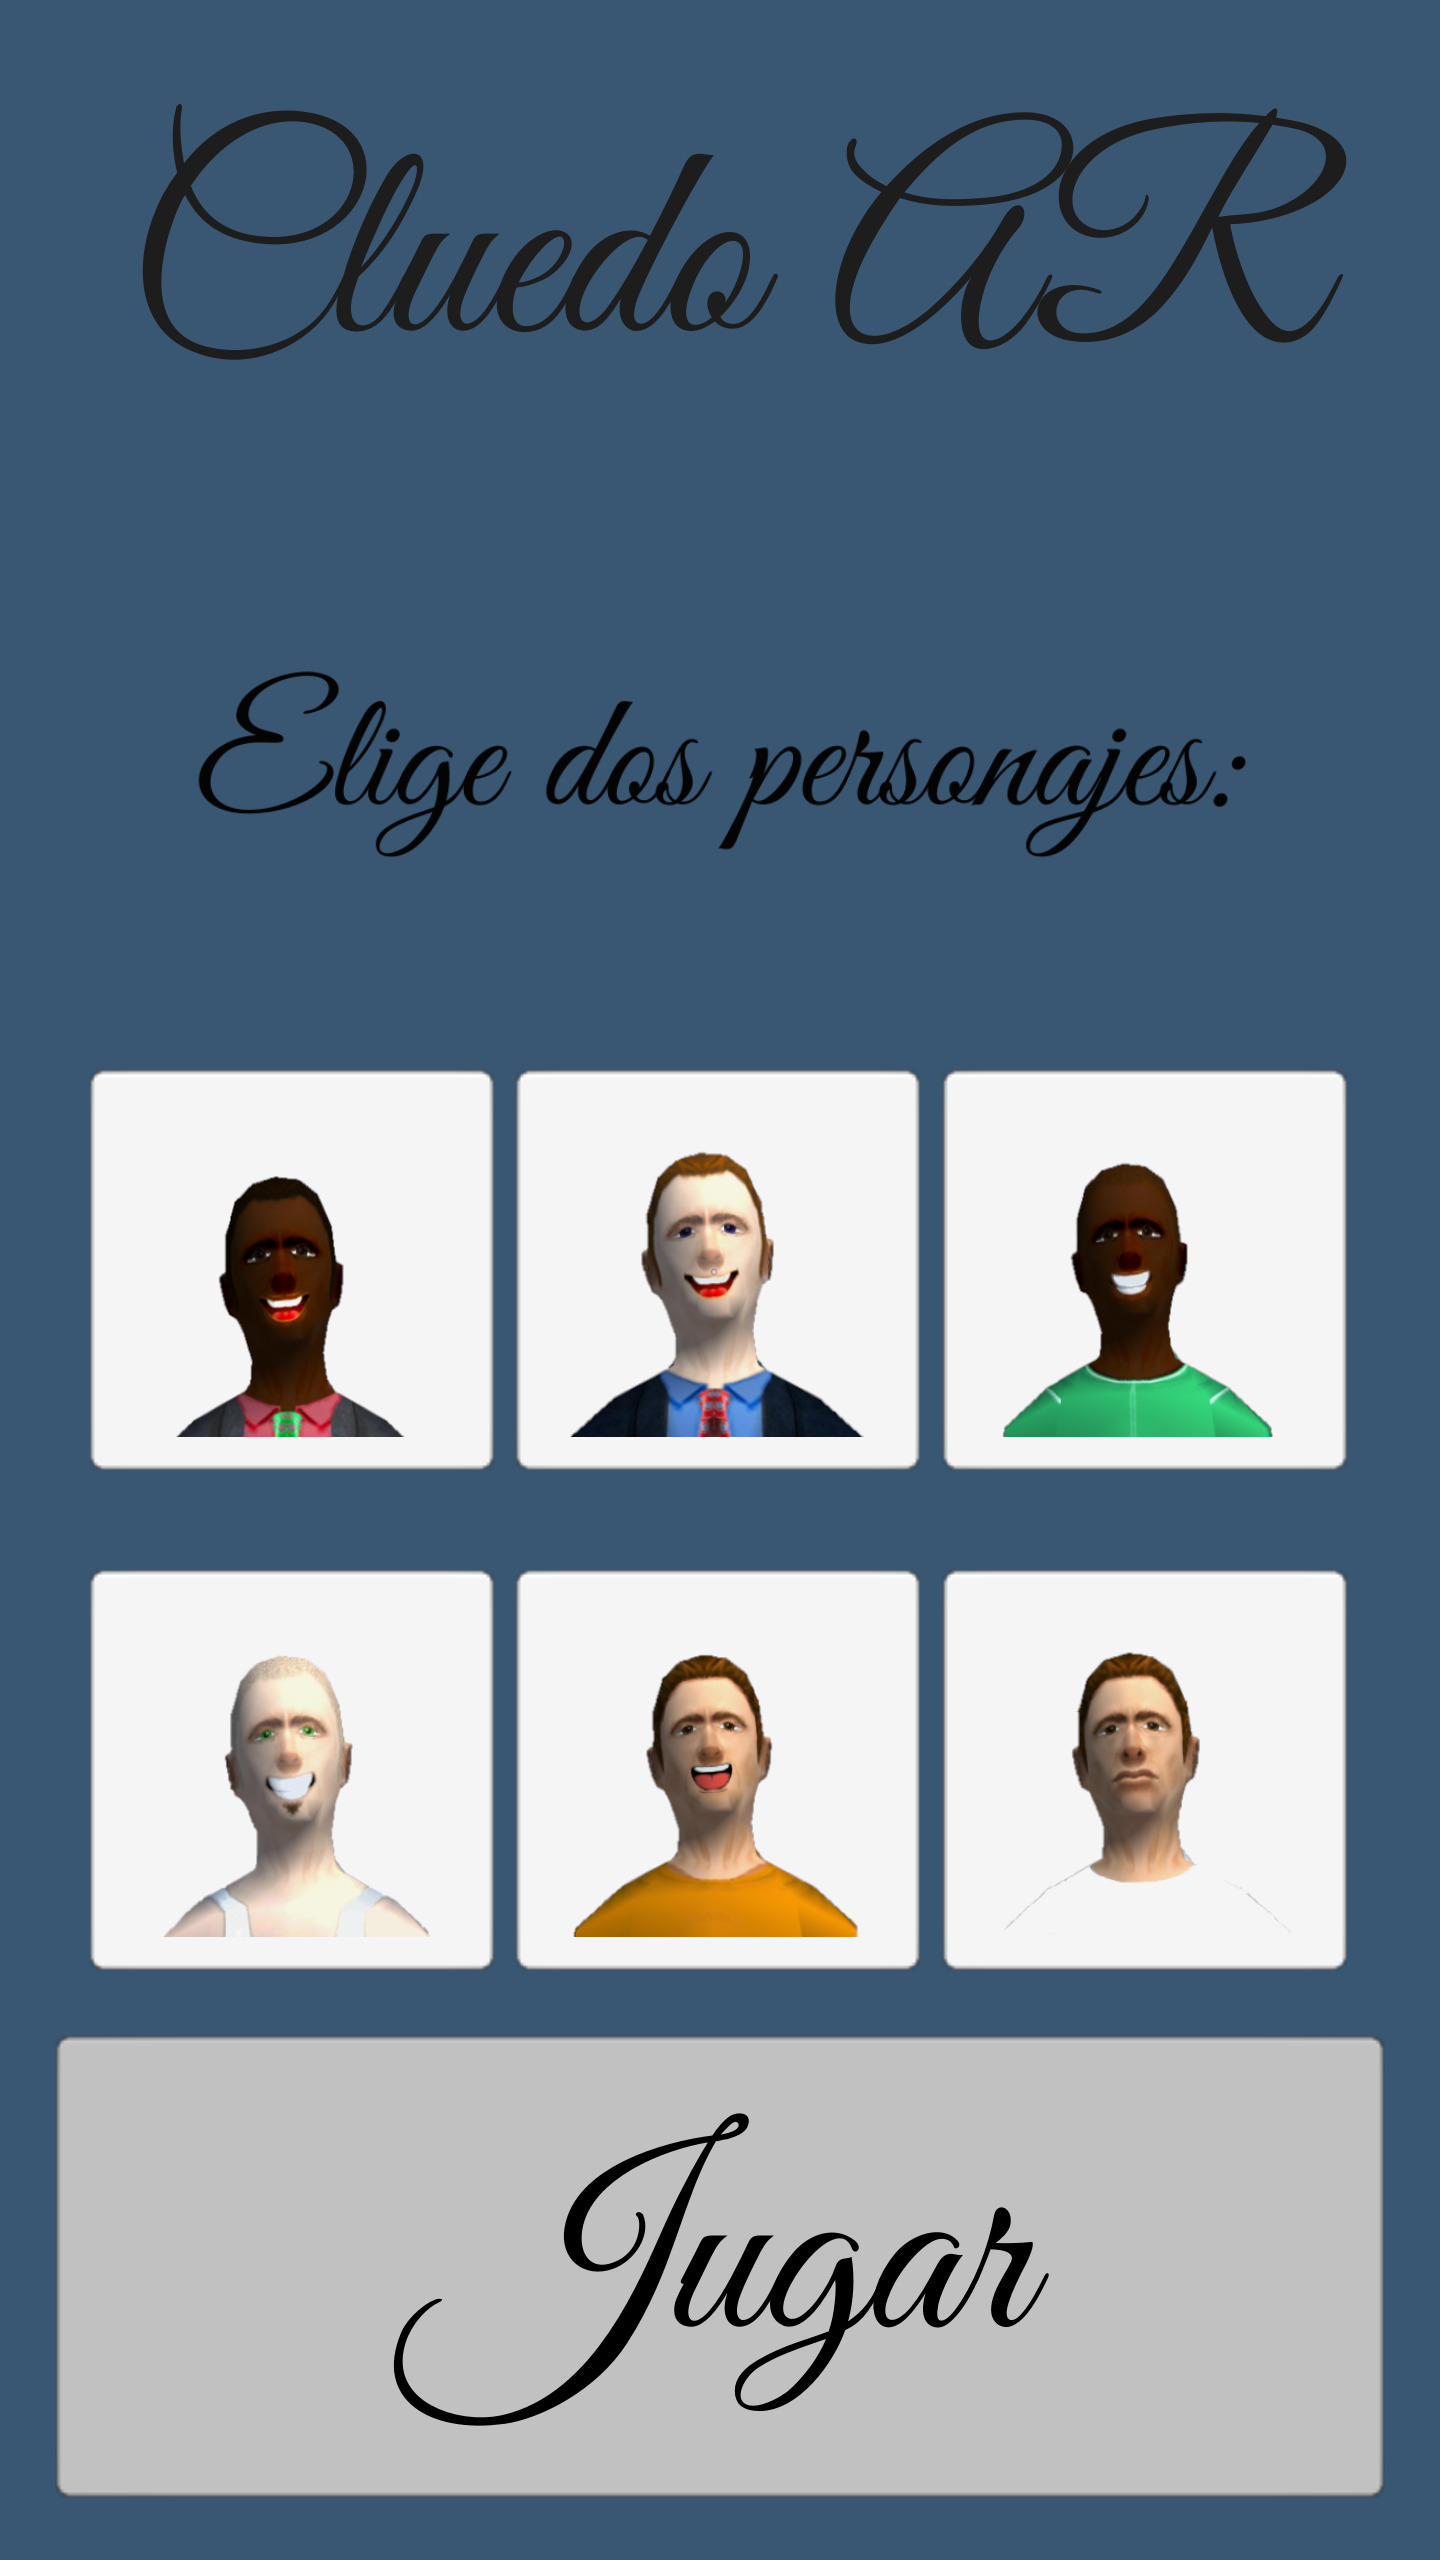
\includegraphics[scale=0.07]{inicial-1}
  \caption{Imagen que muestra la pantalla inicial sin personajes seleccionados.}
  \label{figura-inicial-1}
\end{figure}

Mientras que en la Figura \ref{figura-inicial-2} se puede observar la pantalla de inicio con personajes seleccionados y por tanto el botón de jugar activo.

\begin{figure}[h]
  \centering
  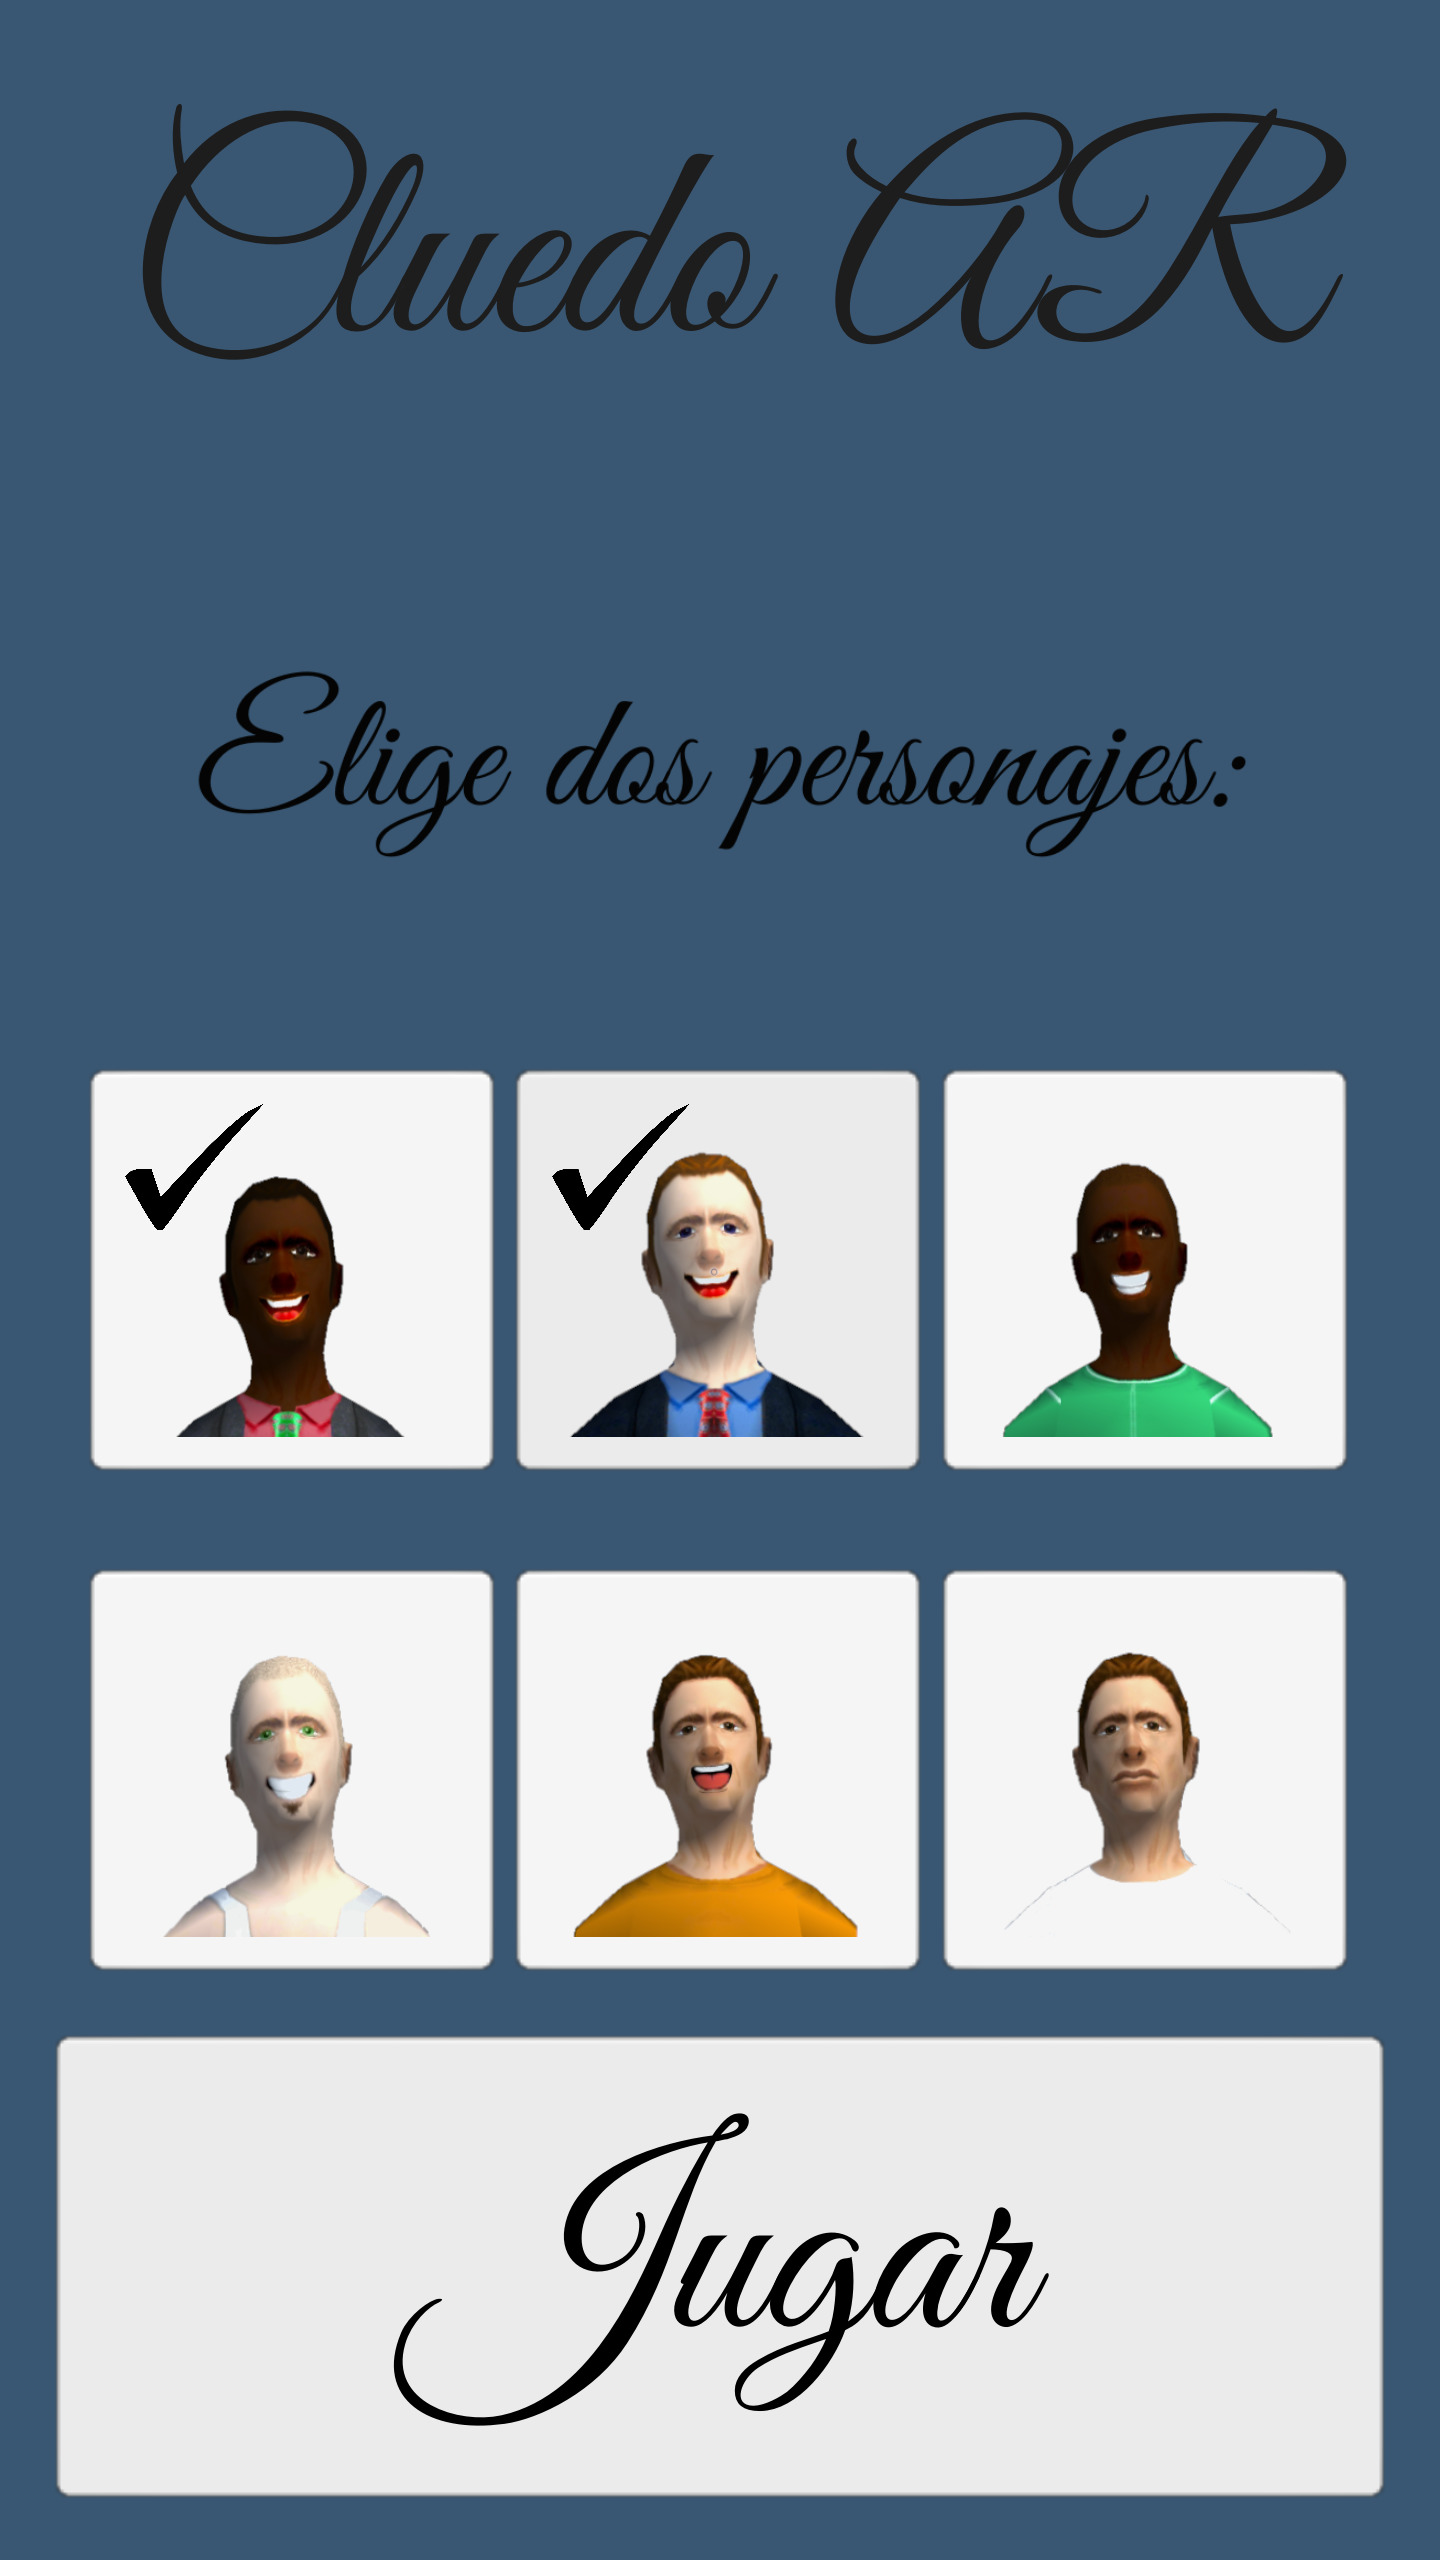
\includegraphics[scale=0.07]{inicial-2}
  \caption{Imagen que muestra la pantalla inicial con personajes seleccionados.}
  \label{figura-inicial-2}
\end{figure}

\newpage

En la Figura \ref{figura-instrucciones} se puede la pantalla de instrucciones.

\begin{figure}[h]
  \centering
  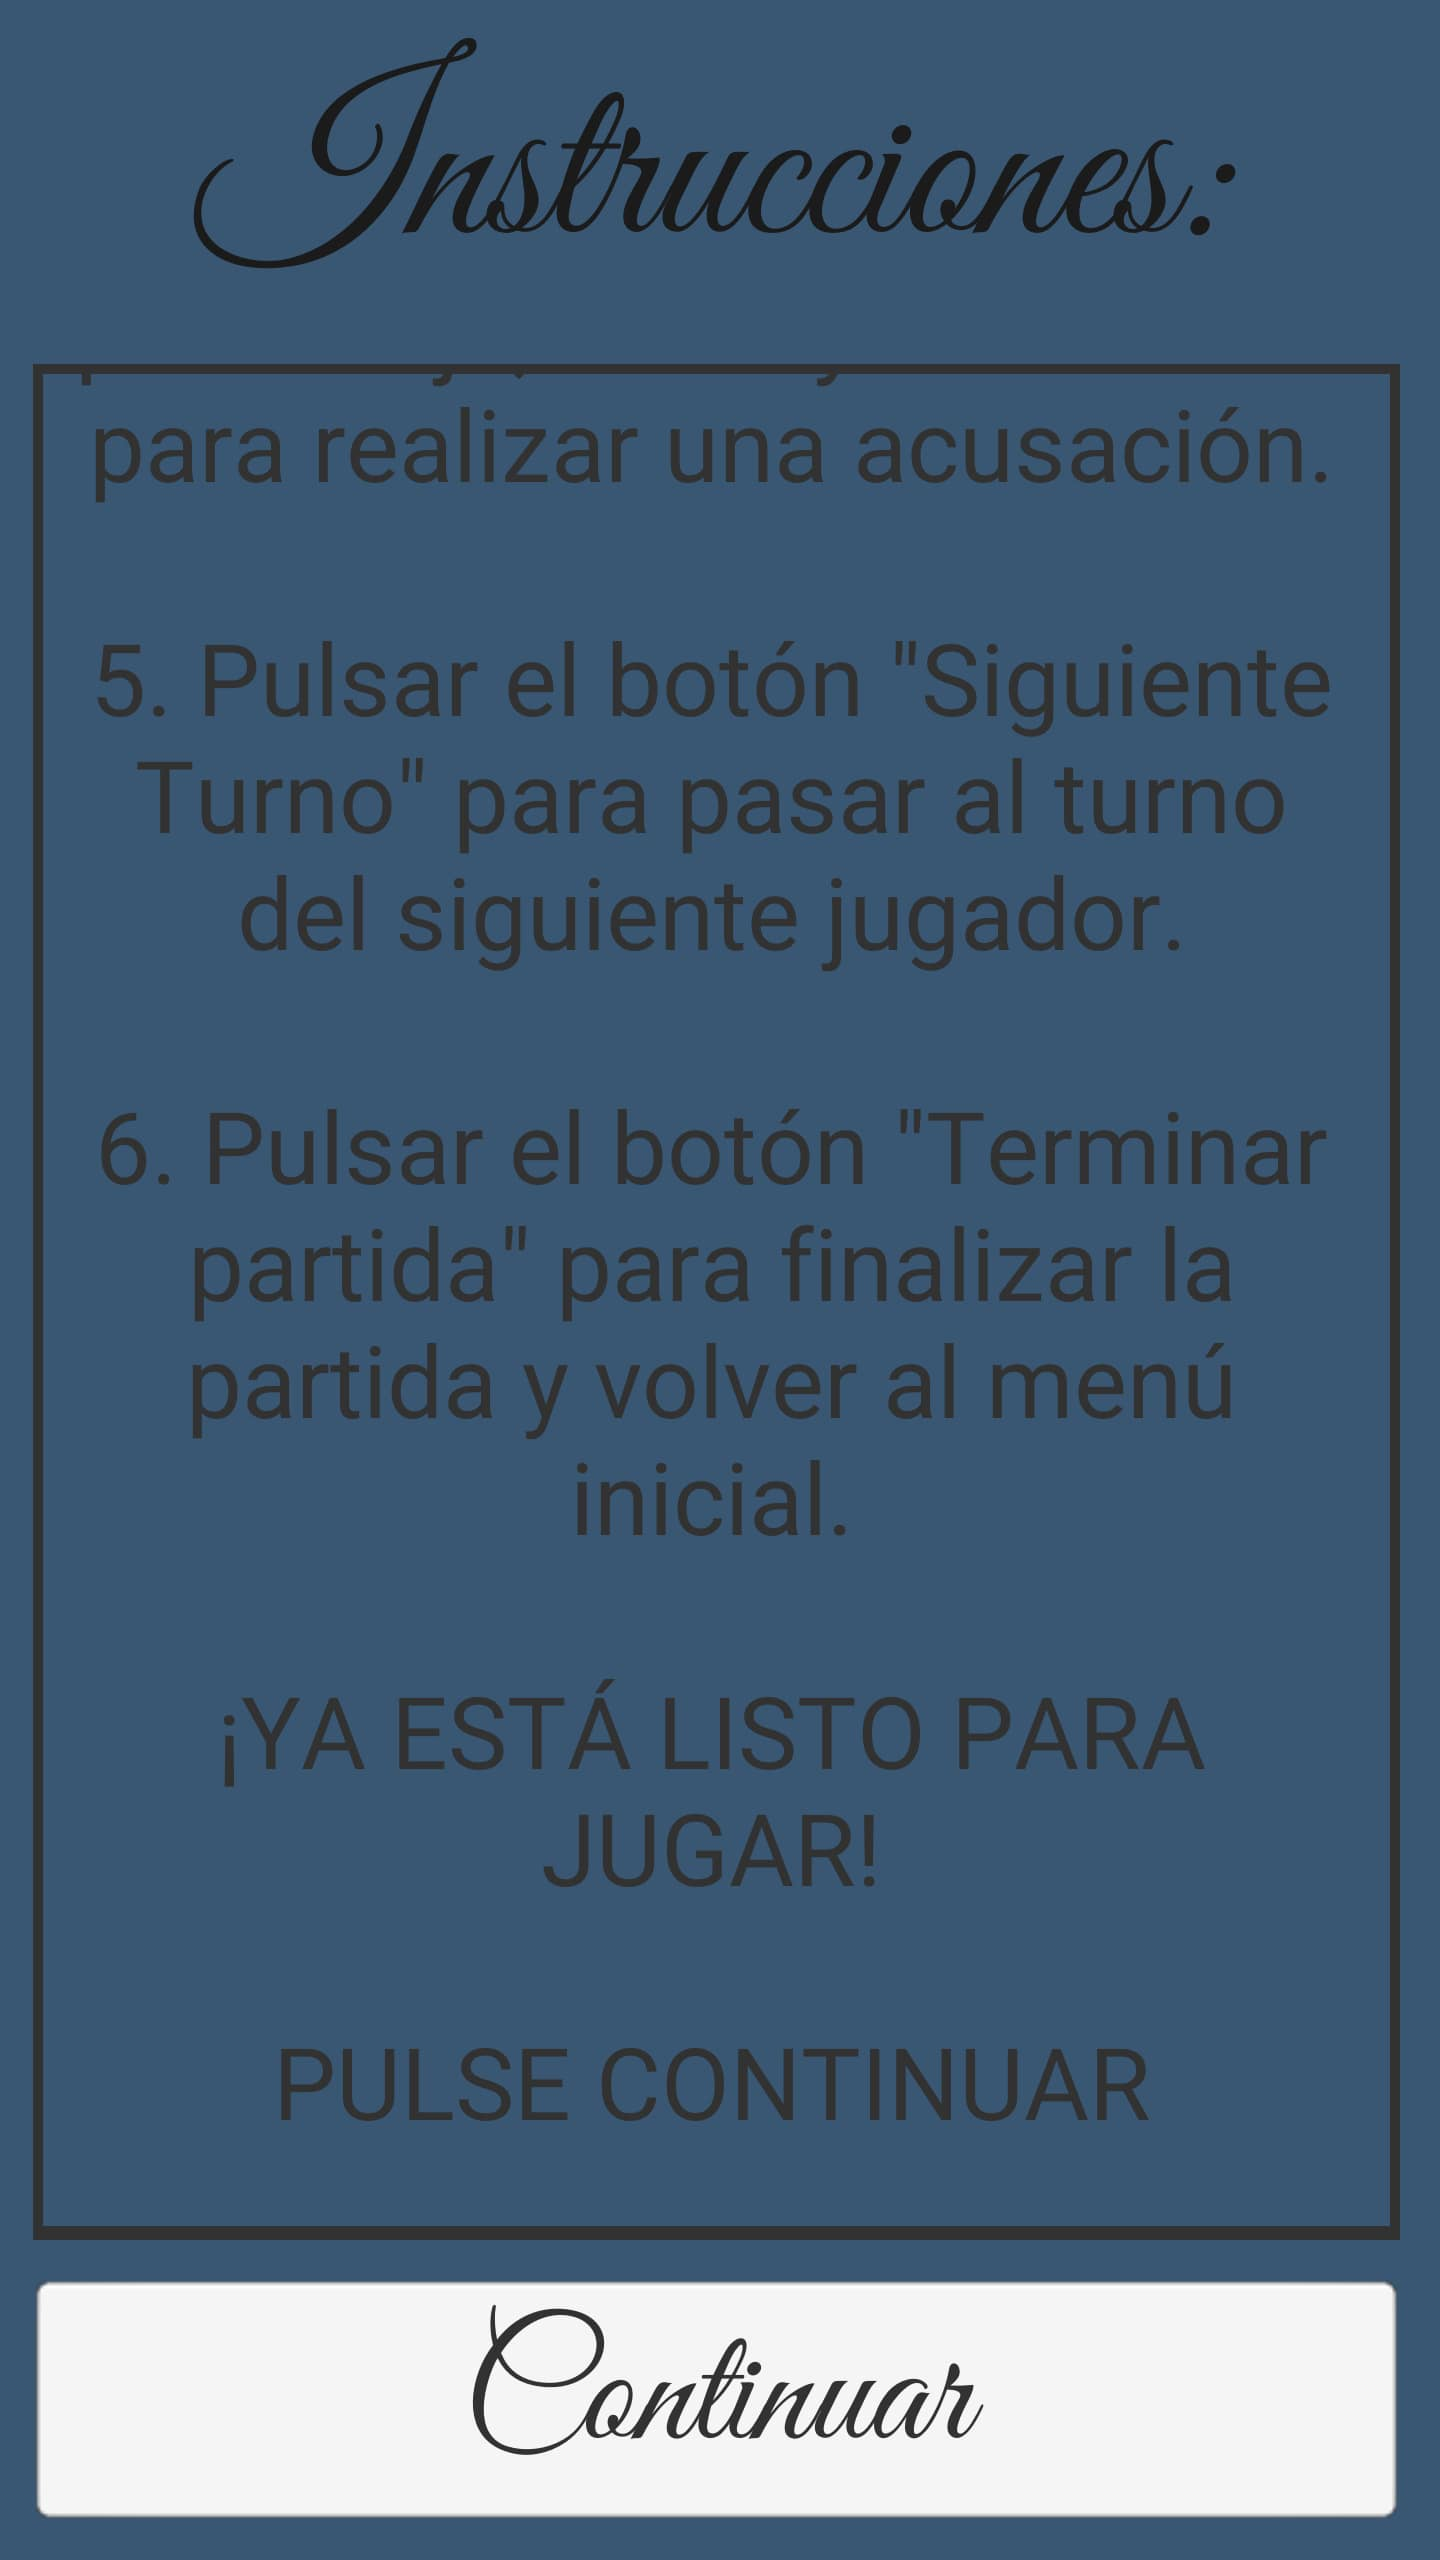
\includegraphics[scale=0.07]{instrucciones}
  \caption{Imagen que muestra la pantalla de instrucciones.}
  \label{figura-instrucciones}
\end{figure}


En la Figura \ref{figura-juego-1} se puede observar la pantalla de juego en con el tablero escaneado, mientras que en la Figura \ref{figura-juego-2} se puede observar mas de cerca como se situan los elementos sobre el tablero, y sobre cada habitación.

\begin{figure}[h]
  \centering
  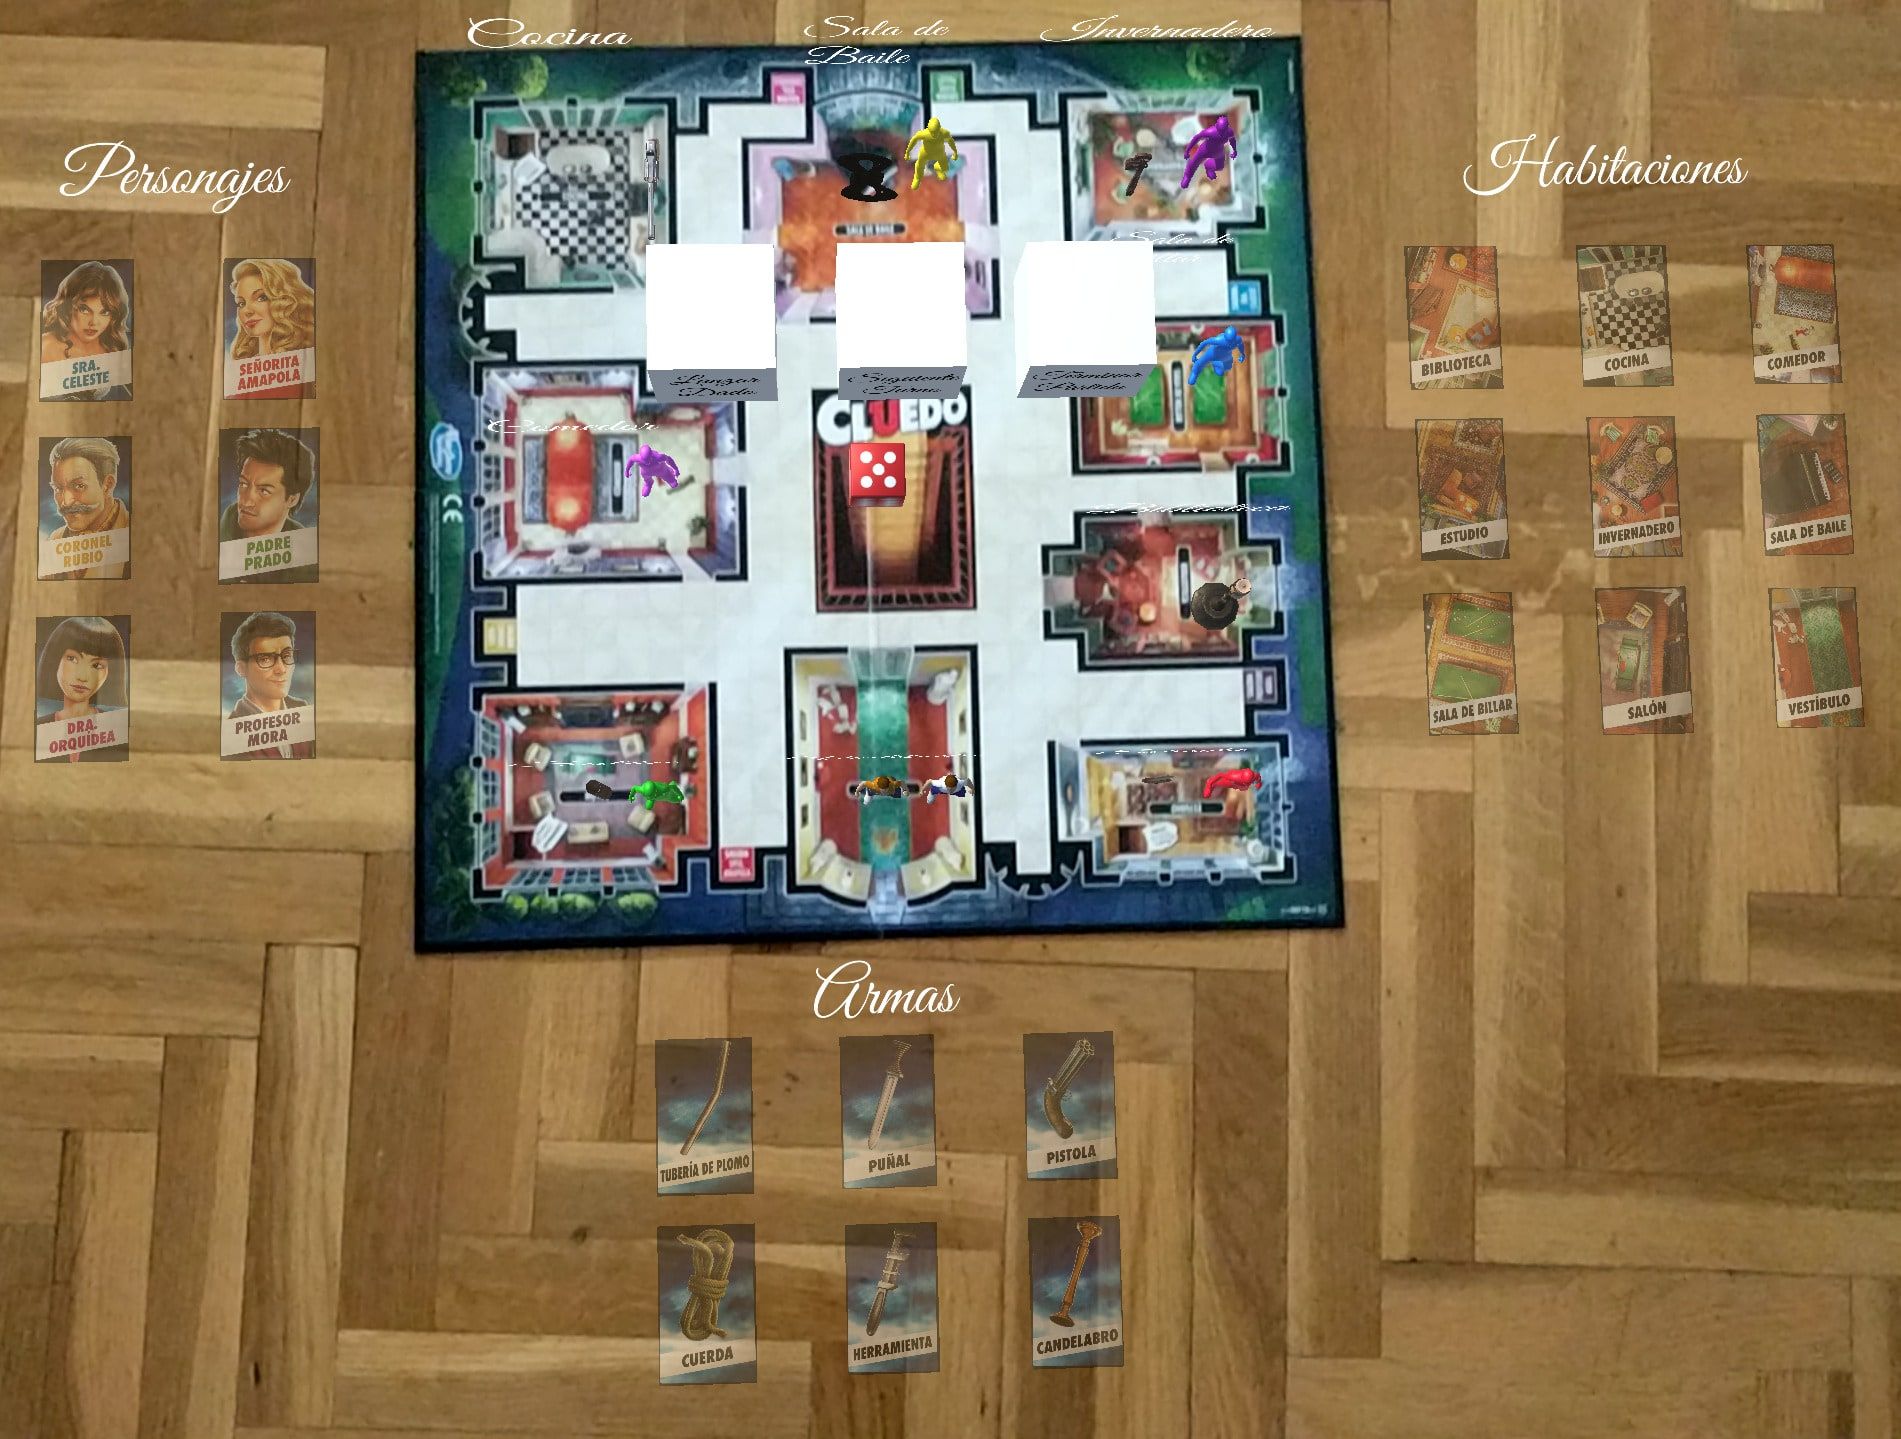
\includegraphics[scale=0.17]{juego-1}
  \caption{Imagen que muestra la pantalla de juego con el tablero escaneado.}
  \label{figura-juego-1}
\end{figure}

\begin{figure}[h]
  \centering
  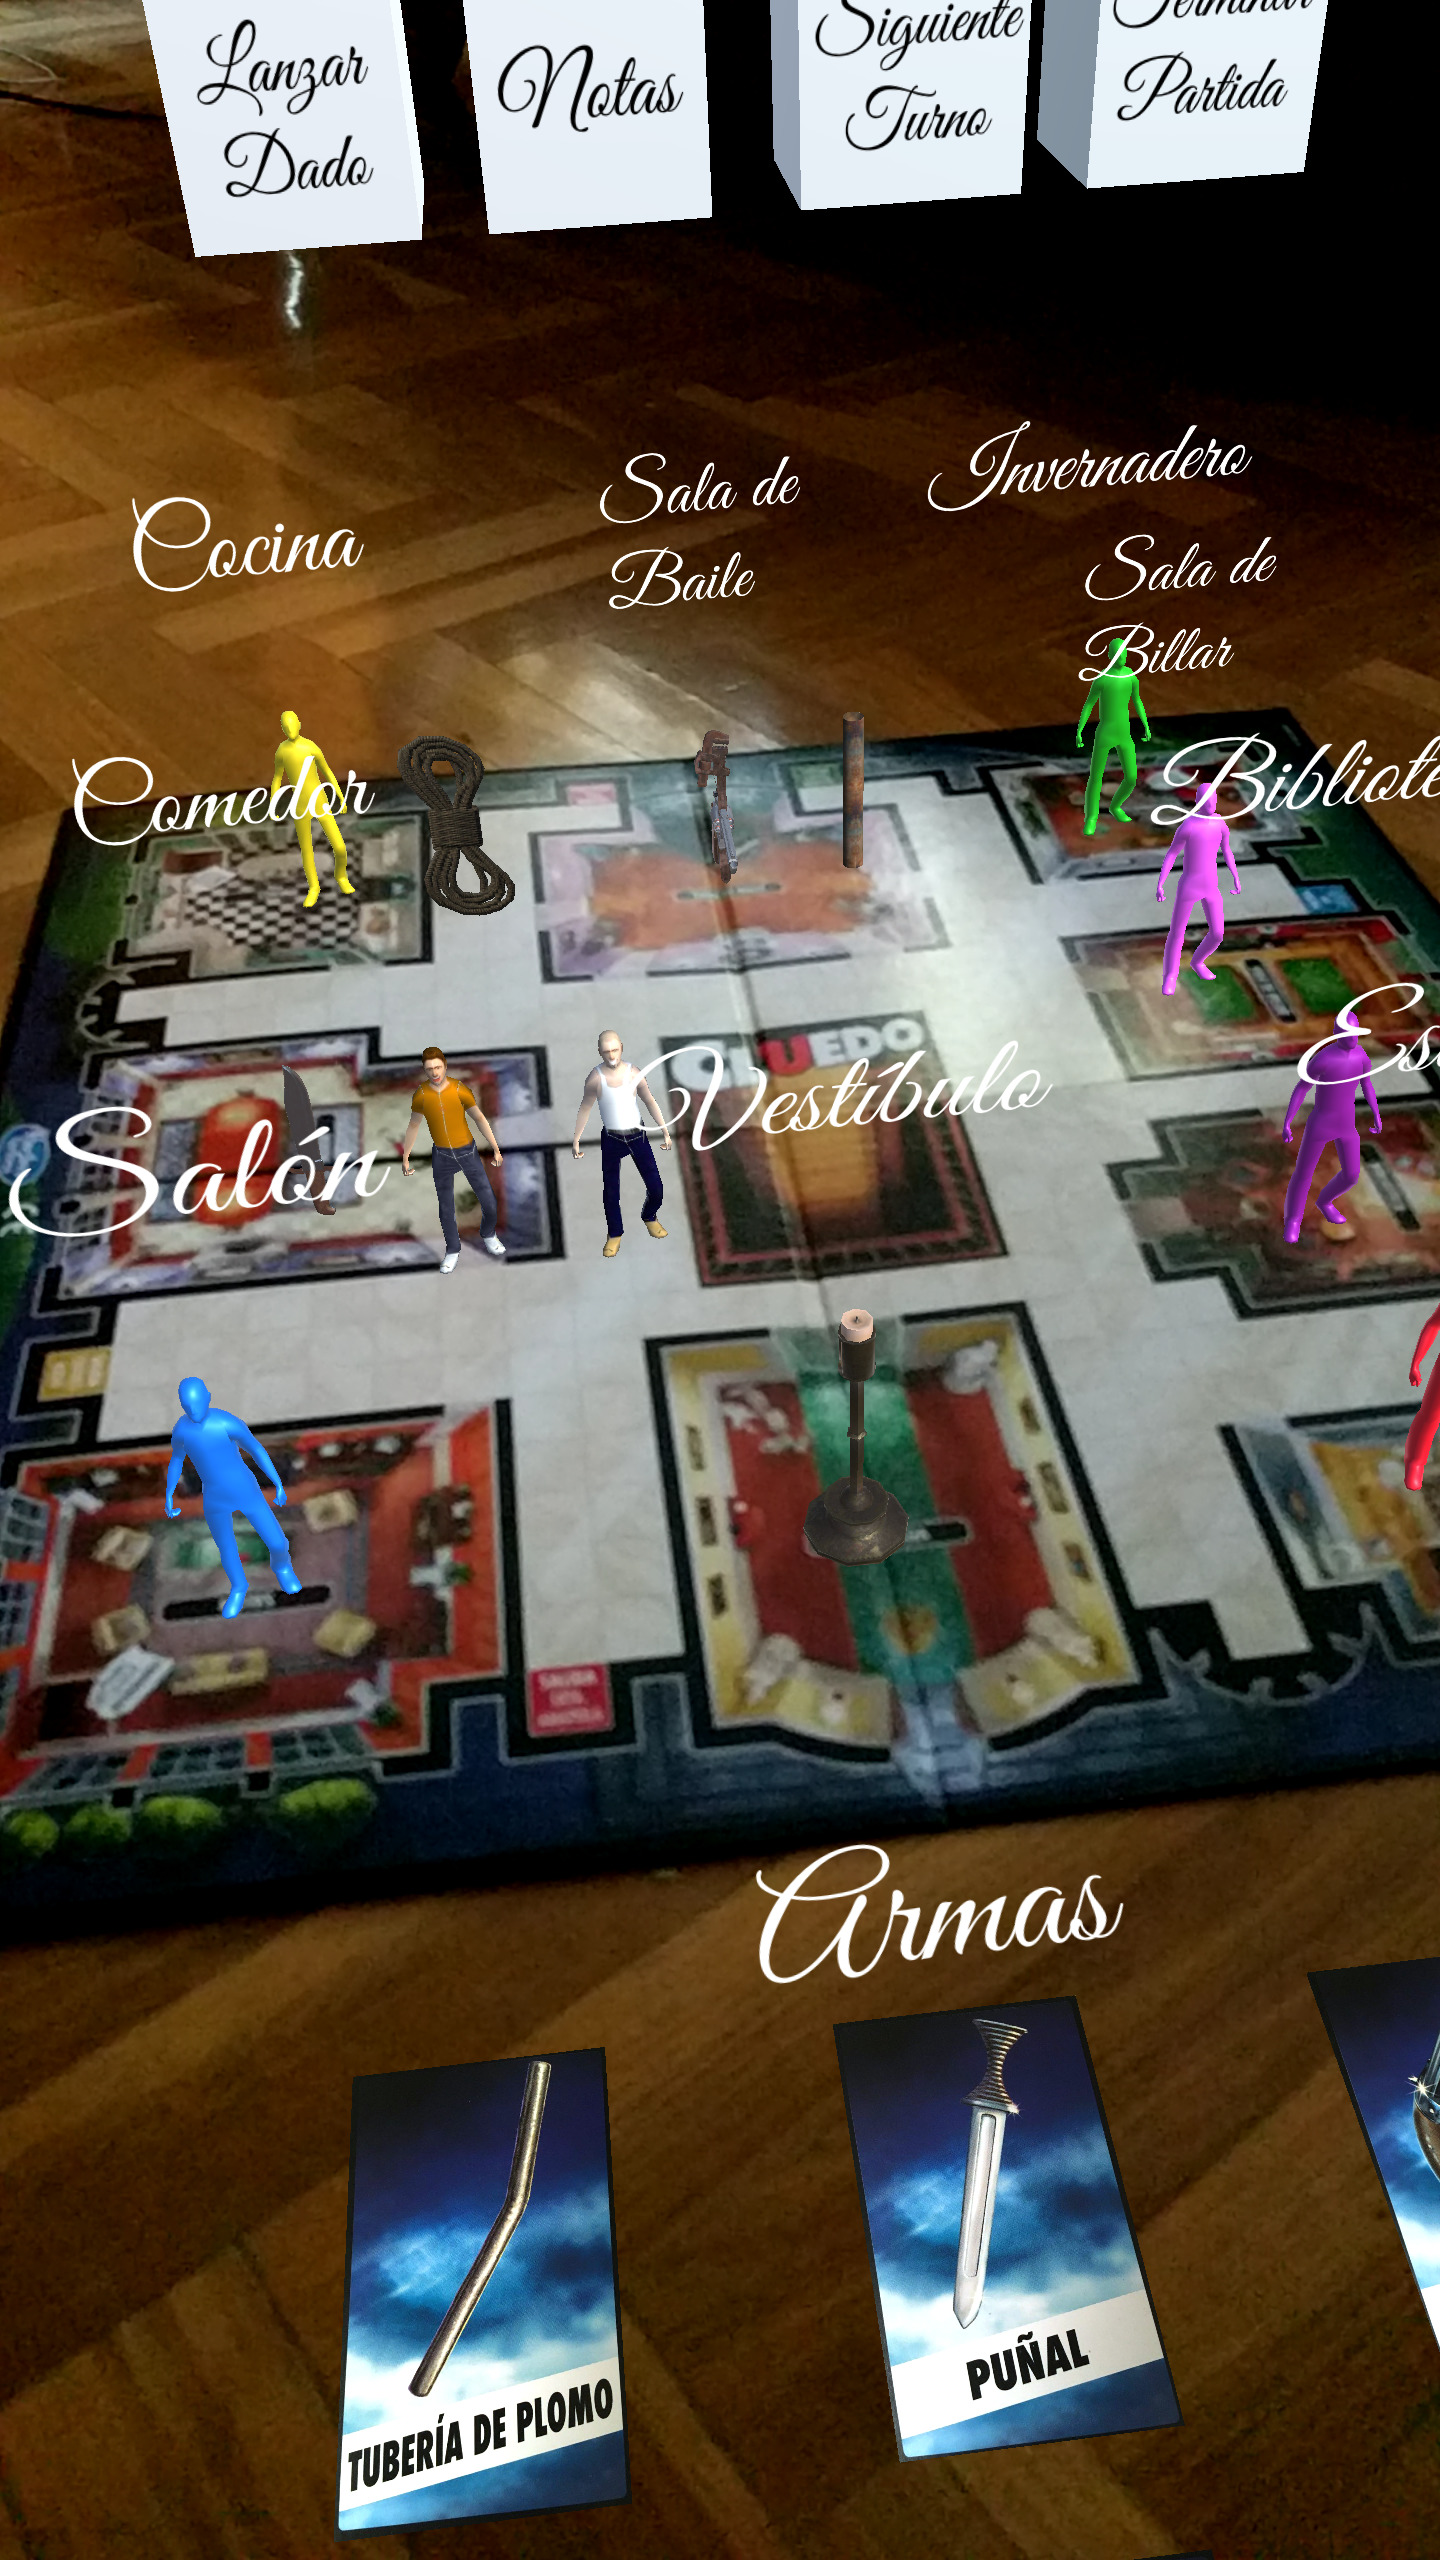
\includegraphics[scale=0.08]{juego-2}
  \caption{Imagen que muestra la pantalla de juego mas de cerca mostrando mas detalles.}
  \label{figura-juego-2}
\end{figure}

\FloatBarrier


\subsection{Tercera iteración}
En esta iteración se han llevado a cabo las historias de usuario \ref{tabla-hu1}, \ref{tabla-hu2} y \ref{tabla-hu3}.\\

En rasgos mas generales, en esta iteración se ha llevado a cabo la pantalla inicial del juego y la pantalla de instrucciones, cuyo resultado se muestra en la \textfb{Entrega 2}.


\subsection{Cuarta iteración}
En esta iteración se ha llevado a cabo la historia de usuario \ref{tabla-hu4}.\\

En rasgos mas generales, en esta iteración se ha llevado a cabo la pantalla de juego que es la pantalla central sobre la que se desarrollará el juego, ya que es la que puede escanear el mundo real, el resultado se muestra en la \textfb{Entrega 2}.\\

Por último, se realizaron pruebas con usuarios, poniendoles en situación se les indicaba la tarea que tenian que hacer, y se fueron apuntando los problemas que estos tenian, detectando así elementos que mejorar en las pantallas de la aplicación realizadas en esta entrega. Los resultados de estas pruebas de usabilidad se encuentran en las Tablas \ref{tabla-entrega-2-usuario1}, \ref{tabla-entrega-2-usuario2} y \ref{tabla-entrega-2-usuario3}.

\subsection{Conclusiones}
Tras la realización de esta entregá se concluye que el proyecto avanza de forma favorable, todas las tareas se han llevado a cabo dentro de plazo y no han surgido grandes problemas.\\

Por otro lado, en las pruebas de usabilidad se comprueba que una vez los usuarios realizan las tareas en el dispositivo móvil en lugar de en los bocetos lo hacen con mas facilidad, ninguno de ellos muestra dificultades a la hora de realizar las tareas solicitadas, por lo que se concluye que el diseño de las pantallas llevadas a cabo en esta entrega se ha realizado de forma exitosa.

\section{Entrega 3}

\subsection{Quinta iteración}
En esta iteración se han llevado a cabo las historias de usuario \ref{tabla-hu5} y \ref{tabla-hu6}.\\

\subsection{Sexta iteración}
En esta iteración se han llevado a cabo las historias de usuario \ref{tabla-hu7} y \ref{tabla-hu8}.\\

\subsection{Séptima iteración}
En esta iteración se han llevado a cabo las historias de usuario \ref{tabla-hu9} y \ref{tabla-hu10}.\\

\section{Entrega 4}

\subsection{Octava iteración}
En esta iteración se ha llevado a cabo la historia de usuario \ref{tabla-hu11}.\\
